\documentclass[11pt,a4paper,twocolumn]{article}

%------------------------------------------------------------------------------
%	REQUIRED PACKAGES AND  CONFIGURATIONS
%------------------------------------------------------------------------------
% PACKAGES FOR TITLES
\usepackage{titlesec}
\usepackage{color}
\usepackage{amsfonts}

% PACKAGES FOR LANGUAGE AND FONT
\usepackage[utf8]{inputenc}
\usepackage[english]{babel}
\usepackage[T1]{fontenc} % Font encoding

% PACKAGES FOR IMAGES
\usepackage{graphicx}
\graphicspath{{Images/}} % Path for images' folder
\usepackage{eso-pic} % For the background picture on the title page
\usepackage{subfig} % Numbered and caption subfigures using \subfloat
\usepackage{caption} % Coloured captions
\usepackage{transparent}

% STANDARD MATH PACKAGES
\usepackage{amsmath}
\usepackage{amsthm}
\usepackage{bm}
\usepackage[overload]{empheq}  % For braced-style systems of equations

% PACKAGES FOR TABLES
\usepackage{tabularx}
\usepackage{longtable} % tables that can span several pages
\usepackage{colortbl}

% PACKAGES FOR ALGORITHMS (PSEUDO-CODE)
\usepackage{algorithm}
\usepackage{algorithmic}
\usepackage{listings}

% PACKAGES FOR REFERENCES & BIBLIOGRAPHY
\usepackage[colorlinks=true,linkcolor=black,anchorcolor=black,citecolor=black,filecolor=black,menucolor=black,runcolor=black,urlcolor=black]{hyperref} % Adds clickable links at references
\usepackage{cleveref}
\usepackage[square, numbers, sort&compress]{natbib} % Square brackets, citing references with numbers, citations sorted by appearance in the text and compressed
\bibliographystyle{plain} % You may use a different style adapted to your field

% PACKAGES FOR THE APPENDIX
\usepackage{appendix}

% PACKAGES FOR ITEMIZE & ENUMERATES 
\usepackage{enumitem}

% OTHER PACKAGES
\usepackage{amsthm,thmtools,xcolor} % Coloured "Theorem"
\usepackage{comment} % Comment part of code
\usepackage{fancyhdr} % Fancy headers and footers
\usepackage{lipsum} % Insert dummy text
\usepackage{tcolorbox} % Create coloured boxes (e.g. the one for the key-words)
\usepackage{stfloats} % Correct position of the tables

%-------------------------------------------------------------------------
%	NEW COMMANDS DEFINED
%-------------------------------------------------------------------------
% EXAMPLES OF NEW COMMANDS -> here you see how to define new commands
\newcommand{\bea}{\begin{eqnarray}} % Shortcut for equation arrays
\newcommand{\eea}{\end{eqnarray}}
\newcommand{\e}[1]{\times 10^{#1}}  % Powers of 10 notation
\newcommand{\mathbbm}[1]{\text{\usefont{U}{bbm}{m}{n}#1}} % From mathbbm.sty
\newcommand{\pdev}[2]{\frac{\partial#1}{\partial#2}}
% NB: you can also override some existing commands with the keyword \renewcommand

%----------------------------------------------------------------------------
%	ADD YOUR PACKAGES (be careful of package interaction)
%----------------------------------------------------------------------------


%----------------------------------------------------------------------------
%	ADD YOUR DEFINITIONS AND COMMANDS (be careful of existing commands)
%----------------------------------------------------------------------------

% Set the geometric layout of the document
\usepackage{geometry}
\geometry{
  top=3cm,
  left = 2.0cm,
  right = 2.0cm,
  bottom=2cm,
  headheight= 2cm,
  headsep= 0cm,
}
\raggedbottom 


% Custom theorem environments
\declaretheoremstyle[
  headfont=\color{black}\normalfont\bfseries,
  bodyfont=\color{black}\normalfont\itshape,
]{colored}

\captionsetup[figure]{labelfont={color=black}} % Set colour of the captions
\captionsetup[table]{labelfont={color=black}} % Set colour of the captions
\captionsetup[algorithm]{labelfont={color=black}} % Set colour of the captions

\theoremstyle{colored}
\newtheorem{theorem}{Theorem}[section]
\newtheorem{proposition}{Proposition}[section]

% Enhances the features of the standard "table" and "tabular" environments.
\newcommand\T{\rule{0pt}{2.6ex}}
\newcommand\B{\rule[-1.2ex]{0pt}{0pt}}

% Algorithm description
\newcounter{algsubstate}
\renewcommand{\thealgsubstate}{\alph{algsubstate}}
\newenvironment{algsubstates}{
    \setcounter{algsubstate}{0}%
    \renewcommand{\STATE}{%
    \stepcounter{algsubstate}%
    \Statex {\small\thealgsubstate:}\space}
    }{}
    
% Custom theorem environment
\newcolumntype{L}[1]{>{\raggedright\let\newline\\\arraybackslash\hspace{0pt}}m{#1}}
\newcolumntype{C}[1]{>{\centering\let\newline\\\arraybackslash\hspace{0pt}}m{#1}}
\newcolumntype{R}[1]{>{\raggedleft\let\newline\\\arraybackslash\hspace{0pt}}m{#1}}

% Custom itemize environment
\setlist[itemize,1]{label=$\bullet$}
\setlist[itemize,2]{label=$\circ$}
\setlist[itemize,3]{label=$-$}
\setlist{nosep}

% Set separation of columns 
\setlength{\columnsep}{30pt}

% Create command for background pic
\newcommand\BackgroundPic{% Adding background picture
	\put(230,358){
		\parbox[b][\paperheight]{\paperwidth}{%
			\vfill
			\centering
			\transparent{0.4}
			\vfill
}}}

% Set indentation
\setlength\parindent{0pt}

% Custom title commands
\titleformat{\section}
{\color{black}\normalfont\Large\bfseries}
{\color{black}\thesection.}{1em}{}
\titlespacing*{\section}
{0pt}{2ex}{1ex}

\titleformat{\subsection}
{\color{black}\normalfont\large\bfseries}
{\color{black}\thesubsection.}{1em}{}
\titlespacing*{\subsection}
{0pt}{2ex}{1ex}

% Custom headers and footers
\pagestyle{fancy}
\fancyhf{}
      
\fancyfoot{}
\fancyfoot[C]{\thepage} % page
\renewcommand{\headrulewidth}{0mm} % headrule width
\renewcommand{\footrulewidth}{0mm} % footrule width

\makeatletter
\patchcmd{\headrule}{\hrule}{\color{black}\hrule}{}{} % headrule
\patchcmd{\footrule}{\hrule}{\color{black}\hrule}{}{} % footrule
\makeatother

% -> Create the header
\chead[C]{
\centering
\textbf{ Executive summary} \hfill \textbf{\author}
\centerline{\rule{1.0\textwidth}{0.4pt}}
}

% -> title of the thesis
\renewcommand{\title}{An FPGA Toolchain for Graph Neural Network Acceleration using High-Level Synthesis}
% -> author name and surname
\renewcommand{\author}{Giovanni Demasi}
% -> MSc course
\newcommand{\course}{Computer Science and Engineering}
% -> advisor name and surname
\newcommand{\advisor}{Prof. Fabrizio Ferrandi}
% co-supervisors
\newcommand{\firstcoadvisor}{Serena Curzel, Michele Fiorito} % insert if any otherwise comment
%\newcommand{\secondcoadvisor}{Name Surname} % insert if any otherwise comment
% -> academic year
\newcommand{\YEAR}{2022-2023}

%-------------------------------------------------------------------------
%	BEGIN OF YOUR DOCUMENT
%-------------------------------------------------------------------------
\begin{document}

%-----------------------------------------------------------------------------
% TITLE PAGE
%-----------------------------------------------------------------------------
% DO NOT REMOVE SPACES BETWEEN LINES!

\twocolumn[{\begin{@twocolumnfalse}

\AddToShipoutPicture*{\BackgroundPic}

\hspace{-0.6cm}
\includegraphics[width=0.6\textwidth]{logo_polimi_ing_indinf_neg.eps}

\vspace{-1mm}
\fontsize{0.3cm}{0.5cm}\selectfont \bfseries \color{black} Executive Summary of the Thesis\\

\vspace{-0.2cm}
\Large{\textbf{\color{black}{\title}}}\\

\vspace{-0.2cm}
\fontsize{0.3cm}{0.5cm}\selectfont \bfseries \color{black} Master of Science in \course\\

\vspace{-0.2cm}
\fontsize{0.3cm}{0.5cm} \selectfont \bfseries Author: \textbf{\author}\\

\vspace{-0.4cm}
\fontsize{0.3cm}{0.5cm}\selectfont \bfseries Advisor: \textbf{\advisor}\\

% if only ONE co-advisor is present:
\vspace{-0.4cm}
\fontsize{0.3cm}{0.5cm}\selectfont \bfseries Co-advisors: \textbf{\firstcoadvisor}\\
% if more than one co-advisors are present:
%\vspace{-0.4cm}
%\fontsize{0.3cm}{0.5cm}\selectfont \bfseries Co-advisors: \textsc{\textbf{\firstcoadvisor}}\textsc{\textbf{\secondcoadvisor}}\\

\vspace{-0.4cm}
\fontsize{0.3cm}{0.5cm}\selectfont \bfseries Academic year: \textsc{\textbf{\YEAR}}

\small \normalfont

\vspace{11pt}

\centerline{\rule{1.0\textwidth}{0.4pt}}

\vspace{15pt}
\end{@twocolumnfalse}}]

\thispagestyle{plain} % In order to not show the header in the first page

%%%%%%%%%%%%%%%%%%%%%%%%%%%%%%%
%%     SUMMARY MAIN TEXT     %%
%%%%%%%%%%%%%%%%%%%%%%%%%%%%%%%

%-----------------------------------------------------------------------------
% INTRODUCTION
%-----------------------------------------------------------------------------
\section{Introduction}
\label{sec:introduction}%

Over the past few years, deep learning has significantly revolutionized various machine learning tasks,
spanning from image classification and video processing to speech recognition and natural language understanding.

A growing number of applications now generate data in the form of complex graphs with intricate relationships and interdependencies among objects.
The inherent complexity of graph data has posed considerable challenges for existing machine learning algorithms.
Consequently, there has been a surge of studies focusing on extending deep learning techniques to accommodate
and leverage graph data.

Graph neural networks (GNNs) have been introduced in response to the growing demand for learning tasks involving
graph data, which encompasses extensive relational information among its elements.
These neural models effectively capture the interdependence among graph nodes by employing message passing mechanisms.

Optimizing and accelerating the capabilities of Graph Neural Networks is necessary due to their increasingly popularity, particularly in domains characterized by vast amounts of data,
such as social networks and chemistry.
In particular, inference in GNNs refers to the time the model takes to make predictions after training.
The duration of the inference process determines the speed at which queries are answered, and researchers strive to minimize this time span.

In applications of deep learning that prioritize low latency, Field-programmable Gate Arrays (FPGAs) outperform other computing devices, such as CPUs and GPUs.
FPGAs offer the advantage of being fine-tuned to the application to strike the optimal balance between power efficiency and meeting performance requirements.
However, the conventional approach to hardware design demands significant effort and relies heavily on the expertise of the designers, leading to varying quality of results.

To address the challenge of accelerating GNNs on FPGAs without having extensive knowledge in hardware design, the objective of this thesis is to develop a comprehensive toolchain that, starting from PyTorch~\cite{DBLP:journals/corr/abs-1912-01703},
a cutting-edge high-level programming framework for creating neural network algorithms based on the Python programming language, enables the
automatic generation of a GNNs FPGA accelerator with minimal effort required.

The toolchain's effectiveness is validated through experimental results, demonstrating significant enhancements in performance.
The generated accelerators improved inference speeds while preserving the accuracy of GNN models.

The main contribution of this thesis is a novel toolchain introduced to accelerate GNN inference, alongside customized optimizations designed to finely enhance model performance.
Part of this research contributed in innovating Torch-MLIR by introducing new compatibility support for PyTorch Geometric.

To accelerate GNN inference, after having identified the main model's bottlenecks, par tof the study consisted in the acceleration of the matrix multiplication by identyfing the best optimizations.
By leveraging the evaluated optimizations, the final outcome of this thesis is a GCN accelerator improving inference speeds.

%-----------------------------------------------------------------------------
% BACKGROUND
%-----------------------------------------------------------------------------

\section{Background}
\label{sec:background}%

\textit{Graphs} are data structures representing a collection of objects, known as vertices or nodes, and a set of edges connecting them.
In a graph, the edges can be either directed or undirected, and they typically connect two vertices, which may or may not be distinct.
The vertices represent entities or elements, and the edges represent their relationships or connections.

Graphs are easy to visualize, but a more formal way is needed when implementing graph algorithms.
The adjacency matrix of a graph provides information about the relationships between nodes in the graph.
It is a matrix of dimensions $N \times N$ where $N$ is the number of nodes in the graph. Each matrix cell is set to 1 if the two nodes are connected, zero otherwise.
A feature vector represents the features or attributes associated with a single entity.

Graph neural networks (GNNs) are deep learning techniques that operate on graph-structured data.
Thanks to their impressive performance, GNNs have recently gained significant popularity as a widely adopted method for graph analysis.

Graph Neural Networks are a group of neural networks which are designed to solve different tasks.
Prediction tasks on graphs can generally be classified into three categories: graph-level, node-level, and edge-level predictions.
In a graph-level task, the objective is to predict the property or characteristic of an entire graph.
Node-level tasks involve predicting the identity or function of individual nodes within a graph.
The remaining prediction task in graphs pertains to edge prediction.

At its core, a GNN is an algorithm that exploits the connectivity within a graph to understand and represent the relationships between nodes.
GNNs consist of multiple interconnected layers and, by relying on the graph's structure, they iteratively processes input edge, vertex, and graph feature vectors, which encode known attributes and transforms them into output feature vectors that capture the desired predictions.

Different popular GNN architectures have been proposed recently, some of which are more suitable for some tasks than others.
The main model used for this thesis is the \textit{Graph Convolutional Network} (GCN)~\cite{DBLP:journals/corr/KipfW16}.

\subsection{Graph Convolutional Network}
\label{subsec:background}%

The core idea behind GCNs is to perform convolution-like operations on the graph, where the convolutional filters are defined based on the graph's adjacency matrix or other graph-specific structures.

Given an undirected graph $\mathcal{G} = (V, E)$, where $V$ represents the set of nodes (vertices), and $E$ represents the set of edges, with an adjacency matrix $\tilde{A}=A+I_N$, where $I_N$ is the identity matrix, the layer-wise propagation rule in a GCN can be expressed as:
\begin{equation}
    \label{eq:gcn_convolution}
    H^{(l+1)} = f \left( \tilde{D}^{-\tfrac{1}{2}}  \tilde{A}  \tilde{D}^{-\tfrac{1}{2}}  H^{(l)}  W^{(l)} \right)
\end{equation}

Where $H^{(l)} \in \mathbb{R} ^{N \times D}$ is the input node features matrix, $W^{(l)}$ is a layer-specific learnable weight matrix, $\tilde{D}$ is the degree matrix defined as $\tilde{D}_{ii} = \sum_{j} \tilde{A}_{ij}$, and $f(\cdot)$ represents a non-linear activation function applied element-wise, such as $ReLU(\cdot) = max(0, \cdot)$.
The Equation~\ref{eq:gcn_convolution} demonstrates the propagation of node features through graph convolution, where the adjacency matrix $\tilde{A}$ captures the connectivity information of the graph, $\tilde{D}^{-\tfrac{1}{2}}$ normalizes the adjacency matrix, and $H^{(l)}  W^{(l)}$ performs a linear transformation of node features.
The resulting $H^{(l+1)}$ represents the updated node representations after the graph convolution operation.

%-----------------------------------------------------------------------------
% PROBLEM FORMULATION
%-----------------------------------------------------------------------------

\section{Problem Formulation}
\label{sec:problem-formulation}%

Graph neural network acceleration refers to designing and implementing hardware accelerators and co-processors to speed up the training or inference of GNNs.
A GNN accelerator aims at optimizing the execution of GNN computations, which involve iterative message-passing between nodes in a graph to update their representations based on neighboring nodes' features.
Hardware acceleration aims to improve the performance, efficiency, and capabilities of computing systems by offloading specific tasks or computations to specialized hardware components.

In particular, this thesis focuses on improving GNNs inference time, by designing specialized hardware to efficiently perform the computation-intensive operations involved in GNNs, such as matrix multiplications, aggregations, and non-linear activation functions.

To explain the potential impact of this thesis's objective, let us consider a recommendation system, in which the goal is to predict what items a user might be interested in based on their past interactions and preferences.
This problem can be represented as a graph, where users items are nodes and interactions between users and items are edges.
A GNN is an optimal choice for modeling recommendation systems, as it can effectively capture relationships and interactions between users and items.
However, as the number of users and items increases, the computational complexity of GNNs can become a significant bottleneck.
One way to address the bottleneck issue is by using a specialized GNN accelerator, which enhances the efficiency and scalability of the recommendation system, resulting in quick and precise recommendations to users.

%-----------------------------------------------------------------------------
% TOOLCHAIN
%-----------------------------------------------------------------------------

\section{Toolchain}
\label{sec:toolchain}%

The main contribution of this thesis is represented by the design of a toolchain for Graph Neural Network acceleration on FPGA leveraging High-Level Synthesis (HLS).
Figure~\ref{fig:toolchain} illustrates the entire design flow, with the steps involved in the GNN acceleration process.

\begin{figure}[t]
    \centering
    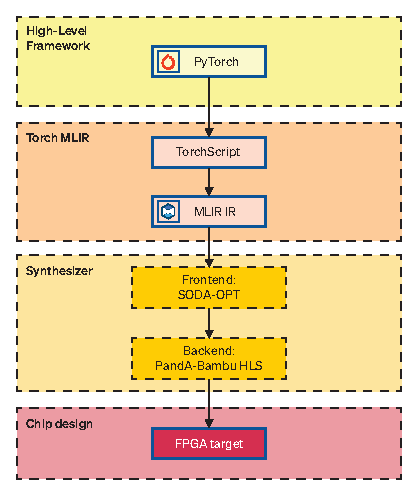
\includegraphics[height=0.36\textwidth]{Images/toolchain}
    \caption{FPGA Toolchain for Graph Neural Network Acceleration}
    \label{fig:toolchain}
\end{figure}

\subsection{PyTorch}
\label{subsec:pytorch-toolchain}%

The first step of the toolchain is to design and implement the Graph Neural Network model in PyTorch~\cite{DBLP:journals/corr/abs-1912-01703}.

The main model used for this thesis is the Graph Convolutional Network~\cite{DBLP:journals/corr/KipfW16} performing node classification on the \textit{Cora} dataset.

\subsection{Torch-MLIR}
\label{subsec:torch-mlir-toolchain}%

Torch-MLIR~\cite{torch_mlir} offers compiler support for transitioning from the PyTorch ecosystem to the MLIR ecosystem.

For this thesis, TorchScript represented the starting point of the flow that Torch-MLIR follows to go from PyTorch to MLIR\@.
TorchScript offers a way to generate serializable and optimizable models directly from PyTorch code.
The TorchScript representation is then converted to MLIR using the built-in conversion of Torch-MLIR.
The result MLIR can use different dialects, but the one used for this thesis is the Linalg dialect, which serves as input for the next phase of the toolchain.

Since Torch-MLIR implicitly uses the TorchScript representation to go from PyTorch to MLIR, the first part of the research consisted of a deep analysis of the Graph Neural Network models to make them compatible with TorchScript.
Some of the used adaptations include making jittable the GNN class, annotate the parameters of the propagate function, using some types assertion and annotate the type of the forward function.

Once having designed, implemented, made compatible with TorchScript, and trained the GNN model in PyTorch, it is possible to use the \lstinline{torch_mlir.compile} API to obtain the MLIR representation of the model.
In particular, this API takes three parameters as input: the GNN model, an input example of the model and the desired output type.
The Graph Neural Network model must have been already trained, being ready for inference.
The second parameter, the input example of the model, is an arbitrary input similar to the one that would be given for inference purposes.
It is required because, by default, the implicit Jit function called by Torch-MLIR to script the model and obtain a script module, involves compiling the forward method and recursively compiling any methods, submodules, and functions called within the forward method. This results in a JIT IR which is converted to the torch dialect which is almost in a 1:1 correspondence.
The torch dialect is then lowered into one of the three available output dialects: linalg, tosa, mhlo.
The purpose of the last parameter is to choose which of these three dialects has to be used for the output MLIR\@.

\subsection{Synthesizer}
\label{subsec:synthesizer-toolchain}%

The synthesizer represents the final step of the toolchain, which optimizes and synthesizes the MLIR representation, targeting FPGA\@.
This step includes SODA-OPT~\cite{9786533} and PandA-Bambu~\cite{9586110}.

\subsubsection*{SODA-OPT}
\label{subsec:soda-opt}%

SODA-OPT receives as input the MLIR representation of the model.
This step is primarily responsible for applying optimizations that can be exploited in the next step.
The output of SODA-OPT is an LLVM representation that serves as input to PandA-Bambu HLS\@.

Once having successfully exported the MLIR representation using the \lstinline{torch_mlir.compile} API, a set of mlir-opt passes have been used to remove the unsupported dialects by lowering them to supported ones,

The next step consists in outlining the part of MLIR code to accelerate by adding the \lstinline{soda.launch} and \lstinline{soda.terminator} flags at the beginning and end of the piece of code.

SODA-OPT provides various passes that can be used to apply optimization to the outlined code.
In particular, it provides a subset of MLIR passes plus a set of passes tailored for soda optimizations.

Profiling the inference function of the GCN model, the result showed that, in general, nearly 60\% of the time required to make a prediction was used for the matrix multiplication operation.
The result of this research showed that the most impressive improvement in terms of performance is given by the loop unrolling technique, which perfectly allows to exploit the extreme parallelism available on FPGAs.

SODA-OPT, after having identified the key code regions, having outlined them into separate MLIR modules, and having applied the transformation passes to the MLIR input, optimizes the portion of code selected for hardware acceleration with a progressive lowering through different MLIR dialects.
As a final result, the input code is translated into an LLVM intermediate representation intentionally restructured for hardware synthesis.

\subsubsection*{PandA-Bambu}
\label{subsec:bambu}%

PandA-Bambu represents the last phase of the synthesis.
It receives the LLVM representation as input, and after having applied some optional low-level optimizations, it performs the typical steps of HLS, including allocation, scheduling and binding.

PandA-Bambu allows the specification of different optimizations and settings that can have a big impact on accelerator performance.
The most evaluated optimization is the number of memory channels.

A comparative analysis has been performed between different number of memory channels, including the minimum, 2 channels, and the maximum, 32 channels.

The LLVM intermediate representation taken as input from PandA-Bambu is received by the Clang compiler frontend which builds an internal IR to perform the HLS steps.
After having applied the specified optimizations, the generated design in an HDL is given as output.

%-----------------------------------------------------------------------------
% EXPERIMENTAL RESULTS
%-----------------------------------------------------------------------------

\section{Experimental Results}
\label{sec:experimental-results}%

All the CPU experiments have been conducted using an Intel Core i9, with 8 cores and a frequency of 2,3 GHz.
On the other hand, the synthesis experiments utilized an AMD Virtex UltraScale+ (Alveo U280) FPGA\@.

The first step to understanding how to accelerate the PyTorch GCN model used was to analyze and profile it.
The results showed that more than 50\% of the self CPU time is used by matrix multiplication.
This result clearly justifies the part of this research dedicated to matrix multiplication acceleration.

\subsection{Matrix multiplication acceleration}
\label{subsec:matmul}%

A first evaluation compared PyTorch times of \lstinline{torch.mm} and the baseline accelerator, showing that the latter is faster for small matrices's sizes, but becomes slower when the sizes of the input matrices increases.

This was an expected result and the following optimizations makes the accelerator able to exploit more parallelism with the aim of deleting this behaviour.

To verify the effectiveness of the proposed optimizations, different comparative analysis have been performed.

\begin{figure}[t]
    \centering
    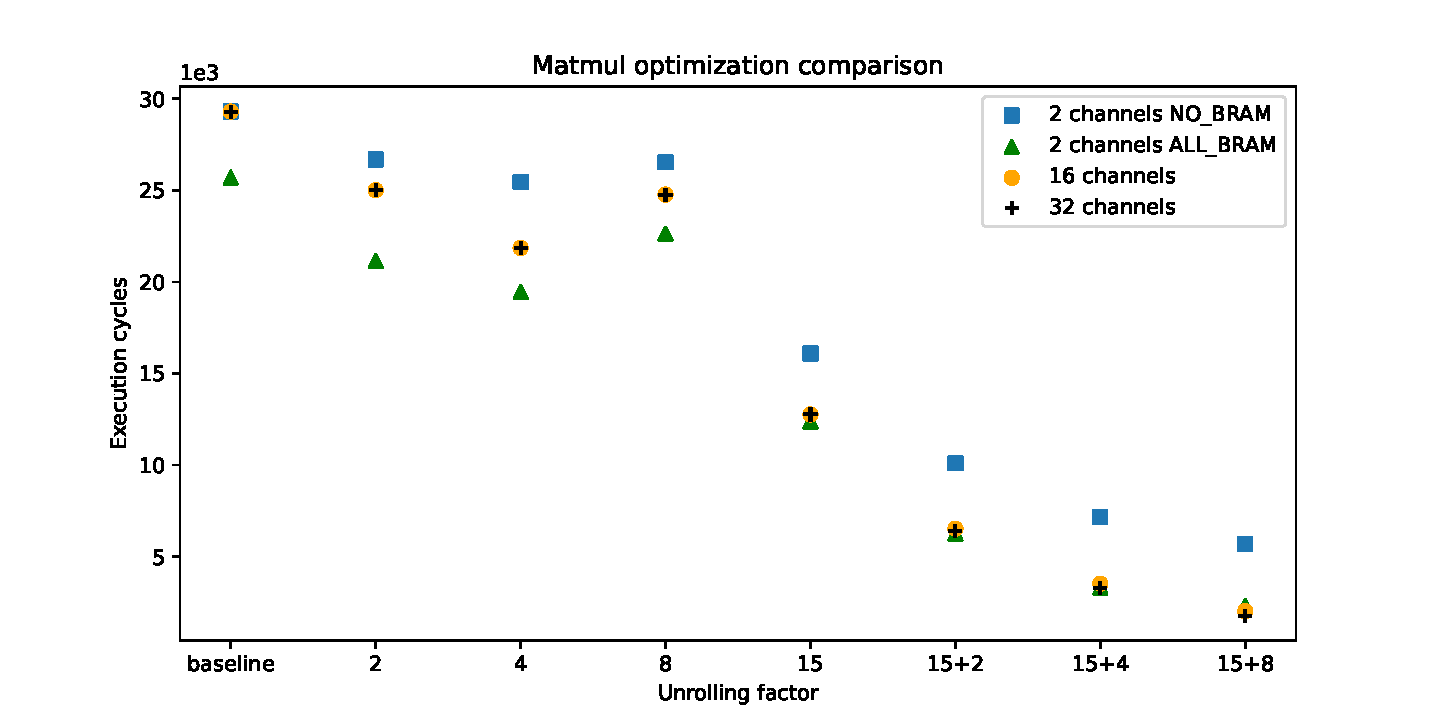
\includegraphics[height=0.24\textwidth]{Images/matmul_comparison15}
    \caption{Matrix multiplication optimization comparison}
    \label{fig:matmul-opts-comparison}
\end{figure}

Figure~\ref{fig:matmul-opt-comparison} shows the impact of the applied optimizations on a matrix multiplication between two matrices of size $15 \times 15$ and $15 \times 16$.
In particular, two different optimizations have been applied: a SODA-OPT progressive loop unrolling, with unrolling factors written in the ordinate of the Figure, and the use of different number of memory channels.
By default, the system employs two channels and utilizes \lstinline{ALL_BRAM} as the memory allocation policy, directing all objects to be stored in BRAMs.
However, the alternative approach explored in this thesis entails employing a greater number of memory channels while utilizing external memory.
To achieve this, the \lstinline{NO_BRAM} memory allocation policy must be selected, leading to all objects being stored in external memory.
This choice offers both advantages and disadvantages, resulting in a trade-off.
Loop unrolling enhances parallelization, thereby reducing computational time.
However, especially when utilizing more than two memory channels, it increases the number of parallel processing elements, leading to a larger area footprint.
Additionally, external memory allows for up to 32 memory channels, enabling the simultaneous loading of 32 variables.
Nonetheless, accessing data from external memory requires more load cycles compared to accessing internal memory.
The conducted analyses aim to highlight the differences among these various configurations, identifying the optimal balance between reducing cycles and containing area utilization.

The most important result is given by the unrolling factor in which the number of cycles needed by the accelerator using 32 memory channels is fewer than the number of cycles needed by the accelerator using 2 memory channels.
The result of this analysis, conducted using different sizes of input matrices, led to the consideration that the number of parallel unrolled loop iterations that justify the use of 32 channels is given by the following equation:
\begin{equation}
    \label{eq:factor-relation}
        i \cdot j \cdot k \geq 2 \cdot \sqrt {M \cdot N \cdot R}
\end{equation}

where $M$, $N$ and $R$ are the sizes of the three nested loops (from the innermost to the outermost), , and $i$, $j$ and $k$ are their respective loop unrolling factors, following the rule $j \neq 1 \iff i=M \land k \neq 1 \iff j=N$.
Equation~\ref{eq:factor-relation} should not be taken as an infallible rule, it is the outcome of this experimental phase and should be used as a general discriminant to decide when to use thirty-two memory channels instead of two.

\subsection{GCN accelerator}
\label{subsec:gcn-accelerator}%

\begin{table}[t]
\centering
    \resizebox{0.45\textwidth}{!}{
    \begin{tabular}{|p{4em} c c c c c|}
    \hline
    \textbf{Name} & \textbf{Nodes} & \textbf{Words} & \textbf{Links} & \textbf{Task} & \textbf{Classes} \T\B \\
    \hline \hline
    \textbf{Cora} & 2708  & 1433 & 5429 & Multiclass classification & 7 \T\B\\
    \hline
    \textbf{Cora15} & 15  & 15 & 3 & Multiclass classification & 7 \T\B\\
    \hline
    \textbf{Cora30} & 30  & 30 & 4 & Multiclass classification & 7 \T\B\\
    \hline
    \textbf{Cora60} & 60  & 60 & 8 & Multiclass classification & 7 \T\B\\
    \hline
    \textbf{Cora90} & 90  & 90 & 18 & Multiclass classification & 7 \T\B\\
    \hline
    \textbf{Cora120} & 120  & 120 & 22 & Multiclass classification & 7 \T\B\\
    \hline
    \textbf{Cora150} & 150  & 150 & 37 & Multiclass classification & 7 \T\B\\
    \hline
    \end{tabular}}
    \\[10pt]
    \caption{Cora sub-dataset used for GCN infernce}
    \label{tab:dataset-definition}
\end{table}

In this Subsection, the ultimate evaluation of the optimizations examined and suggested in the previous Subsection is presented, aimed at understanding their influence on GCN inference time.

Figure~\ref{fig:gcn-inference-comparison} shows the result of a comparative analysis between the PyTorch CPU time and the FPGA accelerator time to perform GCN inference, using different substet of the Cora dataset, as defined in Table~\ref{tab:dataset-definition}.
The PyTorch times have been acquired averaging one million of execution time measurements using the PyTorch built-in benchmark API\@.

\begin{figure}[t]
    \centering
    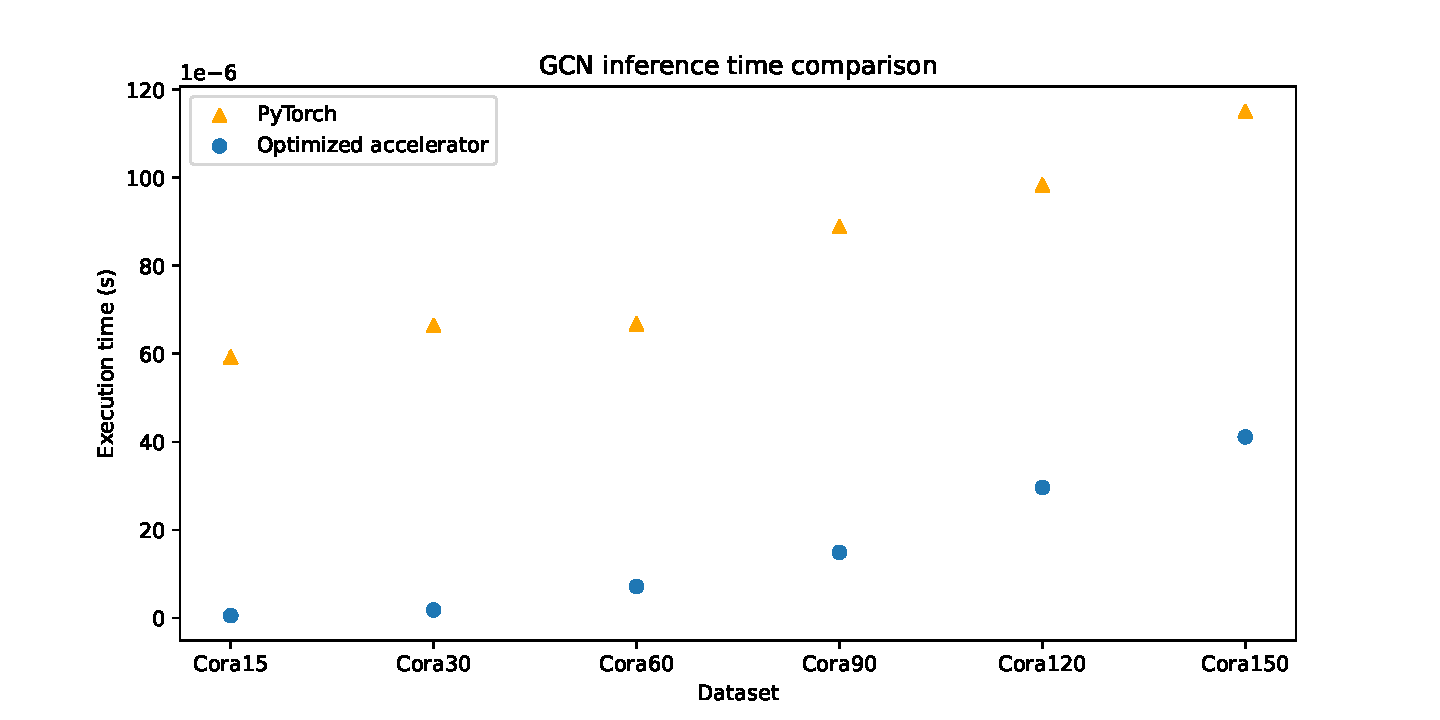
\includegraphics[height=0.24\textwidth]{Images/gcn_forward_comparison}
    \caption{GCN inference time comparison}
    \label{fig:gcn-inference-comparison}
\end{figure}

The results of this final evaluation are incredibly encouraging.
The speedup of the accelerator is not being affected by the size of the input matrices and its computation time is significantly lower with respect to the one measured on CPU with PyTorch.

The area of the accelerator, instead, is obviously affected by the sizes of the input matrices.
This because more the matrices are big, more the parallel loop iterations will be and thus the parallel processing elements.

However, the possibilities offered by the proposed toolchain are various.
It is possible to use less memory channels with a lower loop unrolling factor to still have a big positive impact on performance, but containing the accelerator area requirements.

%-----------------------------------------------------------------------------
% CONCLUSION
%-----------------------------------------------------------------------------
\section{Conclusions}
This thesis tackled the challenge of accelerating Graph Neural Network inference by leveraging High-Level Synthesis techniques targeting FPGAs.

The results of this research significantly contribute to the field of GNN acceleration, introducing a new perspective about how it is possible to obtain hardware accelerators for GNNs even without having any hardware design knowledge.
The toolchain offers different possibilities and provides various optimization passes that can be used in the synthesizer step to fine-tune the accelerator capabilities.

This thesis represents a significant advancement in the field of GNN acceleration.
Nonetheless, there exist opportunities for further enhancement through the implementation of novel features.
Future works could build upon the innovative contributions of this thesis by adding support for new high-level frameworks or by implementing support to sparse tensors.

%---------------------------------------------------------------------------
%  BIBLIOGRAPHY
%---------------------------------------------------------------------------
% essential bibliography
\bibliography{bibliography.bib}

\end{document}